\addcontentsline{toc}{chapter}{Common Programs and Usage}
\chapter*{Common Programs and Usage Notes}
This section is dedicated to solving easy problems using common programs.  

\addcontentsline{toc}{section}{GDAL Binaries}
\section*{GDAL Binaries}

Many of the included gdal programs can be installed using a package manager. 

\begin{description}
\item[Ubuntu] sudo apt-get install gdal-bin
\end{description}

\addcontentsline{toc}{subsection}{gdalinfo}
\subsection*{gdalinfo}

\subsubsection*{Description}
\emph{gdalinfo} is an application bundled with GDAL which provides the user with the ability to extract information about a 
particular geographic file to the console. \index{GDAL} \index{GDAL!gdalinfo} 

This application works on elevation information, vector files (KML, KMZ), imagery (NITF), and many more. 

\noindent\textbf{ Information Provided}
\begin{itemize}
\item Corner Coordinates
\item Geographic Projection Used
\item Image Raster Datatype
\item Date Taken
\item more Metadata and image info
\end{itemize}

\subsubsection*{Usage}
\begin{verbatim}

./gdalinfo  data/dted/w119/n036.dt2

Driver: DTED/DTED Elevation Raster
Files: data/dted/w119/n036.dt2
Size is 3601, 3601
Coordinate System is:
GEOGCS["WGS 84",
    DATUM["WGS_1984",
        SPHEROID["WGS 84",6378137,298.257223563]],
    PRIMEM["Greenwich",0],
    UNIT["degree",0.0174532925199433],
    AUTHORITY["EPSG","4326"]]
Origin = (-119.000138888888884,37.000138888888884)
Pixel Size = (0.000277777777778,-0.000277777777778)
Metadata:
  DTED_VerticalAccuracy_UHL=0007
  DTED_VerticalAccuracy_ACC=0007
  DTED_SecurityCode_UHL=U  
  DTED_SecurityCode_DSI=U
  DTED_UniqueRef_UHL=G18 063     
  DTED_UniqueRef_DSI=G18 063        
  DTED_DataEdition=02
  DTED_MatchMergeVersion=A
  DTED_MaintenanceDate=0000
  DTED_MatchMergeDate=0000
  DTED_MaintenanceDescription=0000
  DTED_Producer=USCNIMA 
  DTED_VerticalDatum=E96
  DTED_HorizontalDatum=WGS84
  DTED_DigitizingSystem=SRTM      
  DTED_CompilationDate=0002
  DTED_HorizontalAccuracy=0013
  DTED_RelHorizontalAccuracy=NA  
  DTED_RelVerticalAccuracy=0009
  AREA_OR_POINT=Point
Corner Coordinates:
Upper Left  (-119.0001389,  37.0001389) (119d 0'0.50"W, 37d 0'0.50"N)
Lower Left  (-119.0001389,  35.9998611) (119d 0'0.50"W, 35d59'59.50"N)
Upper Right (-117.9998611,  37.0001389) (117d59'59.50"W, 37d 0'0.50"N)
Lower Right (-117.9998611,  35.9998611) (117d59'59.50"W, 35d59'59.50"N)
Center      (-118.5000000,  36.5000000) (118d30'0.00"W, 36d30'0.00"N)
Band 1 Block=1x3601 Type=Int16, ColorInterp=Undefined
  NoData Value=-32767
  Unit Type: m

\end{verbatim}

\clearpage
\addcontentsline{toc}{subsection}{gdaldem}
\subsection*{gdaldem}

\subsubsection*{Description}
\emph{gdaldem} is an application bundled with GDAL which provides the user with the ability to 
construct shaded relief and color maps for digital elevation models. \index{GDAL} \index{GDAL!gdaldem} 

This application works on elevation information to include DTED and SRTM.

\subsubsection*{Usage}
\begin{verbatim}

# For color relief maps
gdaldem color-relief data/dted/w118/n36.dt2 color_model.txt output.tif

# For shaded relief maps
gdaldem hillshade  data/dted/w118/n36.dt2 output.tif -s 100000 -z 5

\end{verbatim}
For more information, see manual pages and \url{http://developmentseed.org/blog/2009/jul/30/using-open-source-tools-make-elevation-maps-afghanistan-and-pakistan/}

\begin{figure}[!h]
\subfloat[Color Relief Results]{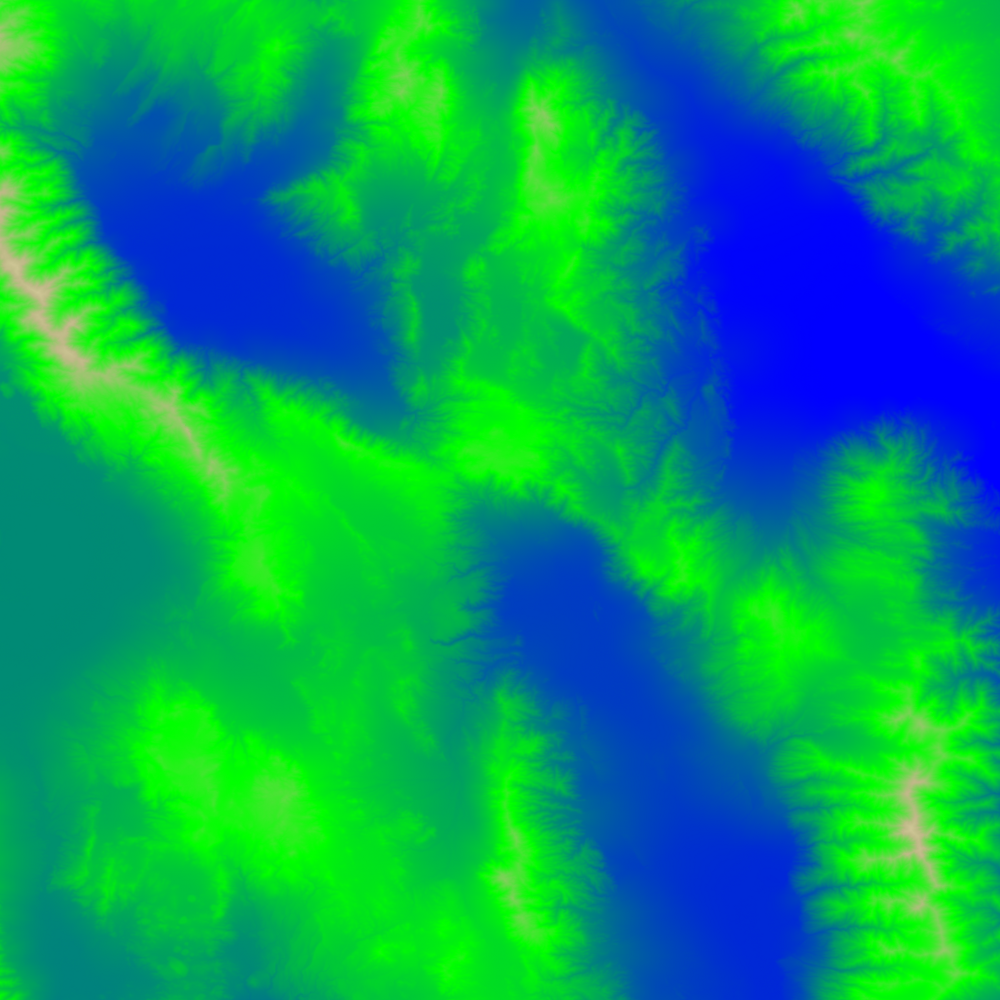
\includegraphics[width=3.5in]{images/color_output.png}}
\subfloat[Hillshade Relief Results]{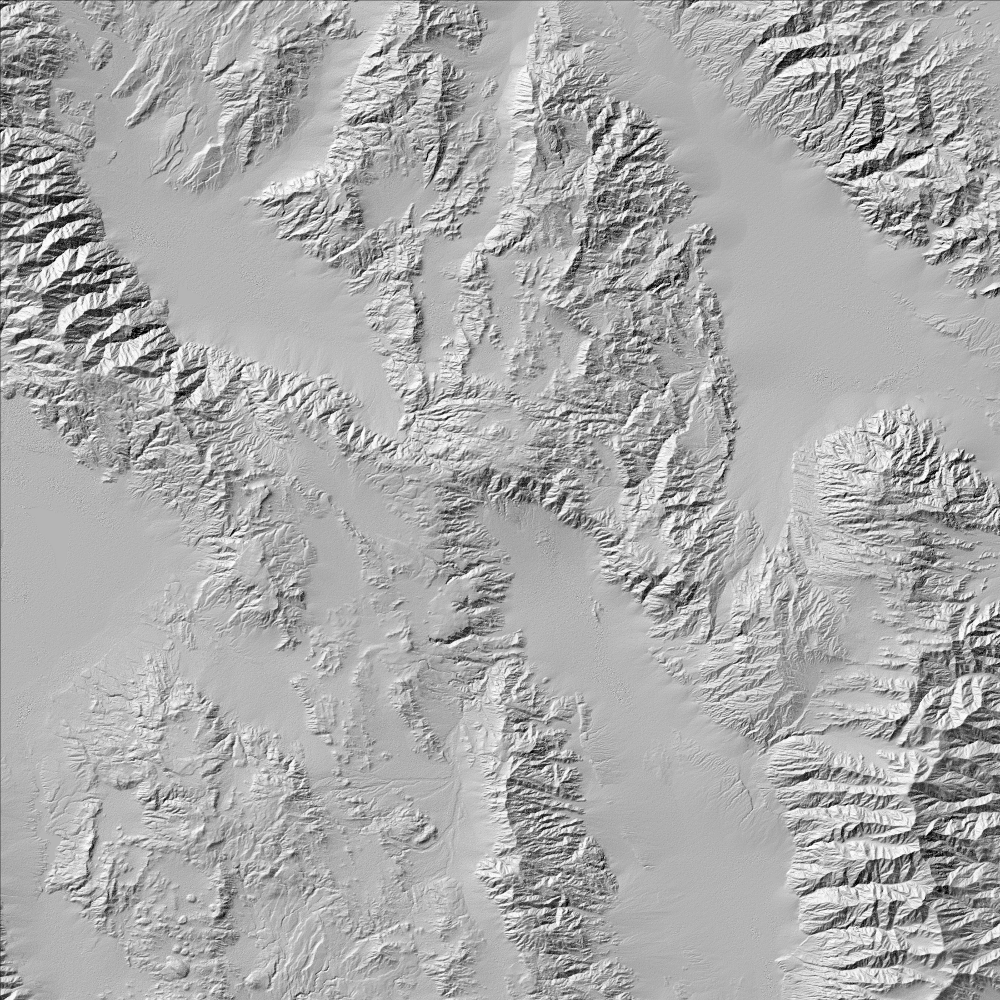
\includegraphics[width=3.5in]{images/hillshade_output.png}}
\caption{Results from typical \emph{gdaldem} usage.}
\label{fig:gdaldem_usage}
\end{figure}

